% -----------------------------------------------------------------
% Document class: Article
\documentclass[ a4paper, twoside, 11pt]{article}
\usepackage{../../../macros-general}
\usepackage{../../../macros-article}
% Number of the handout, quiz, exam, etc.
\newcommand{\numero}{05}
\setcounter{numero}{\numero}

% -----------------------------------------------------------------
\begin{document}
\allowdisplaybreaks

\begin{center}
\Large Mec\'anica Vectorial (MECG-1001): Trabajo Aut\'onomo \numero \\[2ex]
\small \textbf{Semestre:} 2017-2018 T\'ermino II \qquad
\textbf{Instructor:} Luis I. Reyes Castro \qquad
\textbf{Paralelo:} 08
\end{center}
\fullskip

% =============================================
\begin{problem}
\textbf{[4 Puntos]} La barra uniforme $BD$ de 250 mm y 5 kg de masa est\'a conectada como se muestra al disco $A$ y a un collar\'in de masa despreciable, el cual puede deslizarse libremente a lo largo de una barra vertical. Si se sabe que el disco $A$ gira en sentido contrario al de las manecillas del reloj a la velocidad constante de 500 rpm, determine, para el caso cuando $\theta = 90\deg$, \textit{(i)} la aceleraci\'on angular de la barra y \textit{(ii)} la reacci\'on en $D$. 

\begin{figure}[htb]
\centering
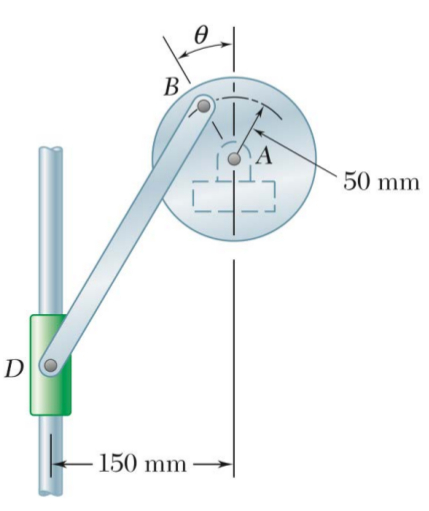
\includegraphics[width=0.4\textwidth]{problema-1.jpg}
\end{figure}

\end{problem}
\fullskip

% =============================================
\begin{problem}
\textbf{[4 Puntos]} La caja uniforme $C$ de 100 kg descansa sobre el piso del elevador donde el coeficiente de fricci\'on est\'atica es $\mu = 0.4$. Determine la mayor aceleraci\'on angular inicial $\alpha$, comenzando desde el reposo en $\theta = 90\deg$, sin causar deslizamiento de la caja. Suponga que no es posible que la caja se vuelque. 

\begin{figure}[htb]
\centering
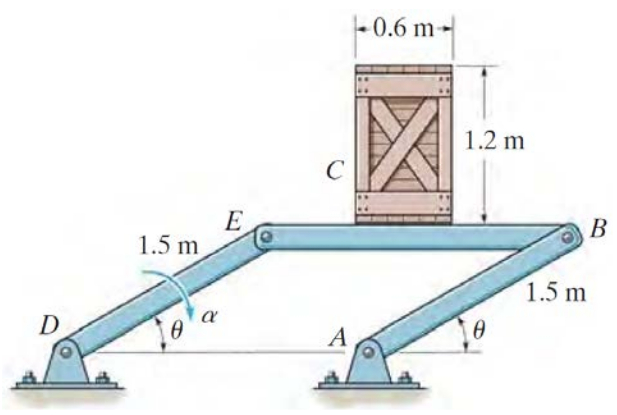
\includegraphics[width=0.6\textwidth]{problema-2.jpg}
\end{figure}

\end{problem}
\fullskip

\end{document}